\documentclass{article}
% Change "article" to "report" to get rid of page number on title page
\usepackage{amsmath,amsfonts,amsthm,amssymb}
\usepackage{setspace}
\usepackage{Tabbing}
\usepackage{fancyhdr}
\usepackage{lastpage}
\usepackage{extramarks}
\usepackage{chngpage}
\usepackage{soul,color}
\usepackage{graphicx,float,wrapfig}
\usepackage{multirow}
\usepackage{enumerate}

% In case you need to adjust margins:
\topmargin=-0.45in      %
\evensidemargin=0in     %
\oddsidemargin=0in      %
\textwidth=6.5in        %
\textheight=9.0in       %
\headsep=0.25in         %

% Homework Specific Information
\newcommand{\hmwkTitle}{Weekly Report III}
\newcommand{\hmwkClass}{}
\newcommand{\hmwkAuthorName}{Donglai\ Wei}


% Setup the header and footer
\pagestyle{fancy}                                                       %
\lhead{\hmwkAuthorName}                                                 %
\rhead{\firstxmark}                                                     %
\lfoot{\lastxmark}                                                      %
\cfoot{}                                                                %
\rfoot{Page\ \thepage\ of\ \pageref{LastPage}}                          %
\renewcommand\headrulewidth{0.4pt}                                      %
\renewcommand\footrulewidth{0.4pt}                                      %

% This is used to trace down (pin point) problems
% in latexing a document:
%\tracingall

%%%%%%%%%%%%%%%%%%%%%%%%%%%%%%%%%%%%%%%%%%%%%%%%%%%%%%%%\begin{enumerate}

% Some tools
\newcommand{\enterProblemHeader}[1]{\nobreak\extramarks{#1}{#1 continued on next page\ldots}\nobreak%
                                    \nobreak\extramarks{#1 (continued)}{#1 continued on next page\ldots}\nobreak}%
\newcommand{\exitProblemHeader}[1]{\nobreak\extramarks{#1 (continued)}{#1 continued on next page\ldots}\nobreak%
                                   \nobreak\extramarks{#1}{}\nobreak}%

\newlength{\labelLength}
\newcommand{\labelAnswer}[2]
  {\settowidth{\labelLength}{#1}%
   \addtolength{\labelLength}{0.25in}%
   \changetext{}{-\labelLength}{}{}{}%
   \noindent\fbox{\begin{minipage}[c]{\columnwidth}#2\end{minipage}}%
   \marginpar{\fbox{#1}}%

   % We put the blank space above in order to make sure this
   % \marginpar gets correctly placed.
   \changetext{}{+\labelLength}{}{}{}}%

\setcounter{secnumdepth}{0}
\newcommand{\homeworkProblemName}{}%
\newcounter{homeworkProblemCounter}%
\newenvironment{homeworkProblem}[1][Problem \arabic{homeworkProblemCounter}]%
  {\stepcounter{homeworkProblemCounter}%
   \renewcommand{\homeworkProblemName}{#1}%
   \section{\homeworkProblemName}%
   \enterProblemHeader{\homeworkProblemName}}%
  {\exitProblemHeader{\homeworkProblemName}}%

\newcommand{\problemAnswer}[1]
  {\noindent\fbox{\begin{minipage}[c]{\columnwidth}#1\end{minipage}}}%

\newcommand{\problemLAnswer}[1]
  {\labelAnswer{\homeworkProblemName}{#1}}

\newcommand{\homeworkSectionName}{}%
\newlength{\homeworkSectionLabelLength}{}%
\newenvironment{homeworkSection}[1]%
  {% We put this space here to make sure we're not connected to the above.
   % Otherwise the changetext can do funny things to the other margin

   \renewcommand{\homeworkSectionName}{#1}%
   \settowidth{\homeworkSectionLabelLength}{\homeworkSectionName}%
   \addtolength{\homeworkSectionLabelLength}{0.25in}%
   \changetext{}{-\homeworkSectionLabelLength}{}{}{}%
   \subsection{\homeworkSectionName}%
   \enterProblemHeader{\homeworkProblemName\ [\homeworkSectionName]}}%
  {\enterProblemHeader{\homeworkProblemName}%

   % We put the blank space above in order to make sure this margin
   % change doesn't happen too soon (otherwise \sectionAnswer's can
   % get ugly about their \marginpar placement.
   \changetext{}{+\homeworkSectionLabelLength}{}{}{}}%

\newcommand{\sectionAnswer}[1]
  {% We put this space here to make sure we're disconnected from the previous
   % passage

   \noindent\fbox{\begin{minipage}[c]{\columnwidth}#1\end{minipage}}%
   \enterProblemHeader{\homeworkProblemName}\exitProblemHeader{\homeworkProblemName}%
   \marginpar{\fbox{\homeworkSectionName}}%

   % We put the blank space above in order to make sure this
   % \marginpar gets correctly placed.
   }%

%%%%%%%%%%%%%%%%%%%%%%%%%%%%%%%%%%%%%%%%%%%%%%%%%%%%%%%%%%%%%



%%%%%%%%%%%%%%%%%%%%%%%%%%%%%%%%%%%%%%%%%%%%%%%%%%%%%%%%%%%%%
% Make title
\title{\vspace{0.3in}\textmd{\textbf{\hmwkTitle}}}
\date{2010.5.4}
\author{\textbf{\hmwkAuthorName}}
%%%%%%%%%%%%%%%%%%%%%%%%%%%%%%%%%%%%%%%%%%%%%%%%%%%%%%%%%%%%%

\begin{document}
\begin{spacing}{1.1}
\maketitle



  
\section{1. HDP Gaussian Mixture Model}
\large {\bf 0) Notation:}\\
 \underline{Observations:}\\
  $\ \ \vec x=(x_{(11)},...,x_{(JN_{j})})$ J Restaurants,$N_{j}$ customers for each   \\
 \underline{Hidden Variables}:\\
  $\ \ \vec z$: assignments of table for customers($\vec t$) and dish for tables($\vec k$) from HDP;\\    
  $\ \ \theta$: mean($\mu$) and covariance matrix($\Omega$) of Gaussian distributions;\\ 
 \underline{Hyperparameters}:\\
 $\ \ \lambda$:($m_{0},B_{0},\eta_{0},\xi_{0}$ for $\mu,\Omega$ and $\alpha,\gamma$ for $\vec z$) \\ \\ 
\large {\bf 1) Graphical Model for HDP:}\\
\begin{center}
    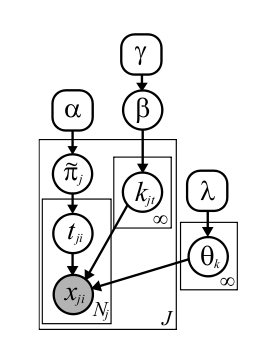
\includegraphics[width=3in,height=4in]{hdp.jpg} 
\end{center}
\large {\bf 2) Generative Model:}\\
Likelihood Term:\\ 
$p(x_{n},\theta|\lambda,z_{n})=\mathcal{N}(x_{n}|z_{n},\mu,\Omega)
\mathcal{N}(\mu|m_{0},\xi_{0}\Omega)\mathcal{W}(\Omega|\eta_{0},B_{0})$\\ 
Allocation Term:\\ 
$p(\vec z|\lambda)=\Pi_{j=1}^{J}[\frac{\Gamma(\alpha)}{\Gamma(n_{j..}+\alpha)}\Pi_{t=1}^{m_{j.}}(\Gamma(n_{jt.}))]\alpha^{\sum_{j=1}^{J}m_{j.}}
\times \frac{\Gamma(\gamma)}{\Gamma(T+\gamma)}\Pi_{k=1}^{K} [\Gamma(m_{.k})] \gamma^{K}$ \\ \\ \\
\large {\bf 3) Marginal Probability given $\vec z$:}\\
Margianlizing out $\theta$,we get the negative of the log probability:\\ \\
 $log(p(x|z,\lambda))$:\\=
(Likelihood)$ -\sum_{k=1}^{K} [\frac{D n_{..k}}{2}log\pi+\frac{D}{2}log\frac{\xi_{k}}{\xi_{0}}+\frac{\eta_{k}}{2}log det(B_{k})-\frac{\eta_{0}}{2}log det(B_{0})
-log \frac{\Gamma_{D}(\frac{\eta_{k}}{2})}{\Gamma_{D}(\frac{\eta_{0}}{2})}]$
\\
-
\\
(Allocation:)$\underline{\sum_{j=1}^{J}\sum_{t=1}^{m_{j.}}[\frac{1}{m_{j.}}log \frac{\Gamma(n_{j..}+\alpha)}{\Gamma(\alpha)} -log(\Gamma(n_{jt.})-log \alpha]+
 \sum_{k=1}^{K} [\frac{1}{K}log \frac{\Gamma(T+\gamma)}{\Gamma(\gamma)} -log(\Gamma(m_{.k})-log \gamma]}$
\\ \\ \\ \\ \\ \\ \\ \\ \\ \\
\section{2. Toy Data Set}

\subsection{0) Setting}

\begin{enumerate}[(I)]
\item 9 Restaurants,200 customers for each,
\item Generate the table assignment for each customer from a Dirichlet Process(concentration parameter $\alpha$) in each restaurant.
\item Generate the dish assignment for each table from a Dirichlet Process (concentration parameter $\gamma$)
\item Generate datas for each dish from one of the pre-defined 14 seperated 2-D Gaussian 
\end{enumerate}
\subsection{1) Ground Truth}
\begin{figure}[h] 
  \begin{minipage}[b]{0.5\textwidth} 
    \centering 
        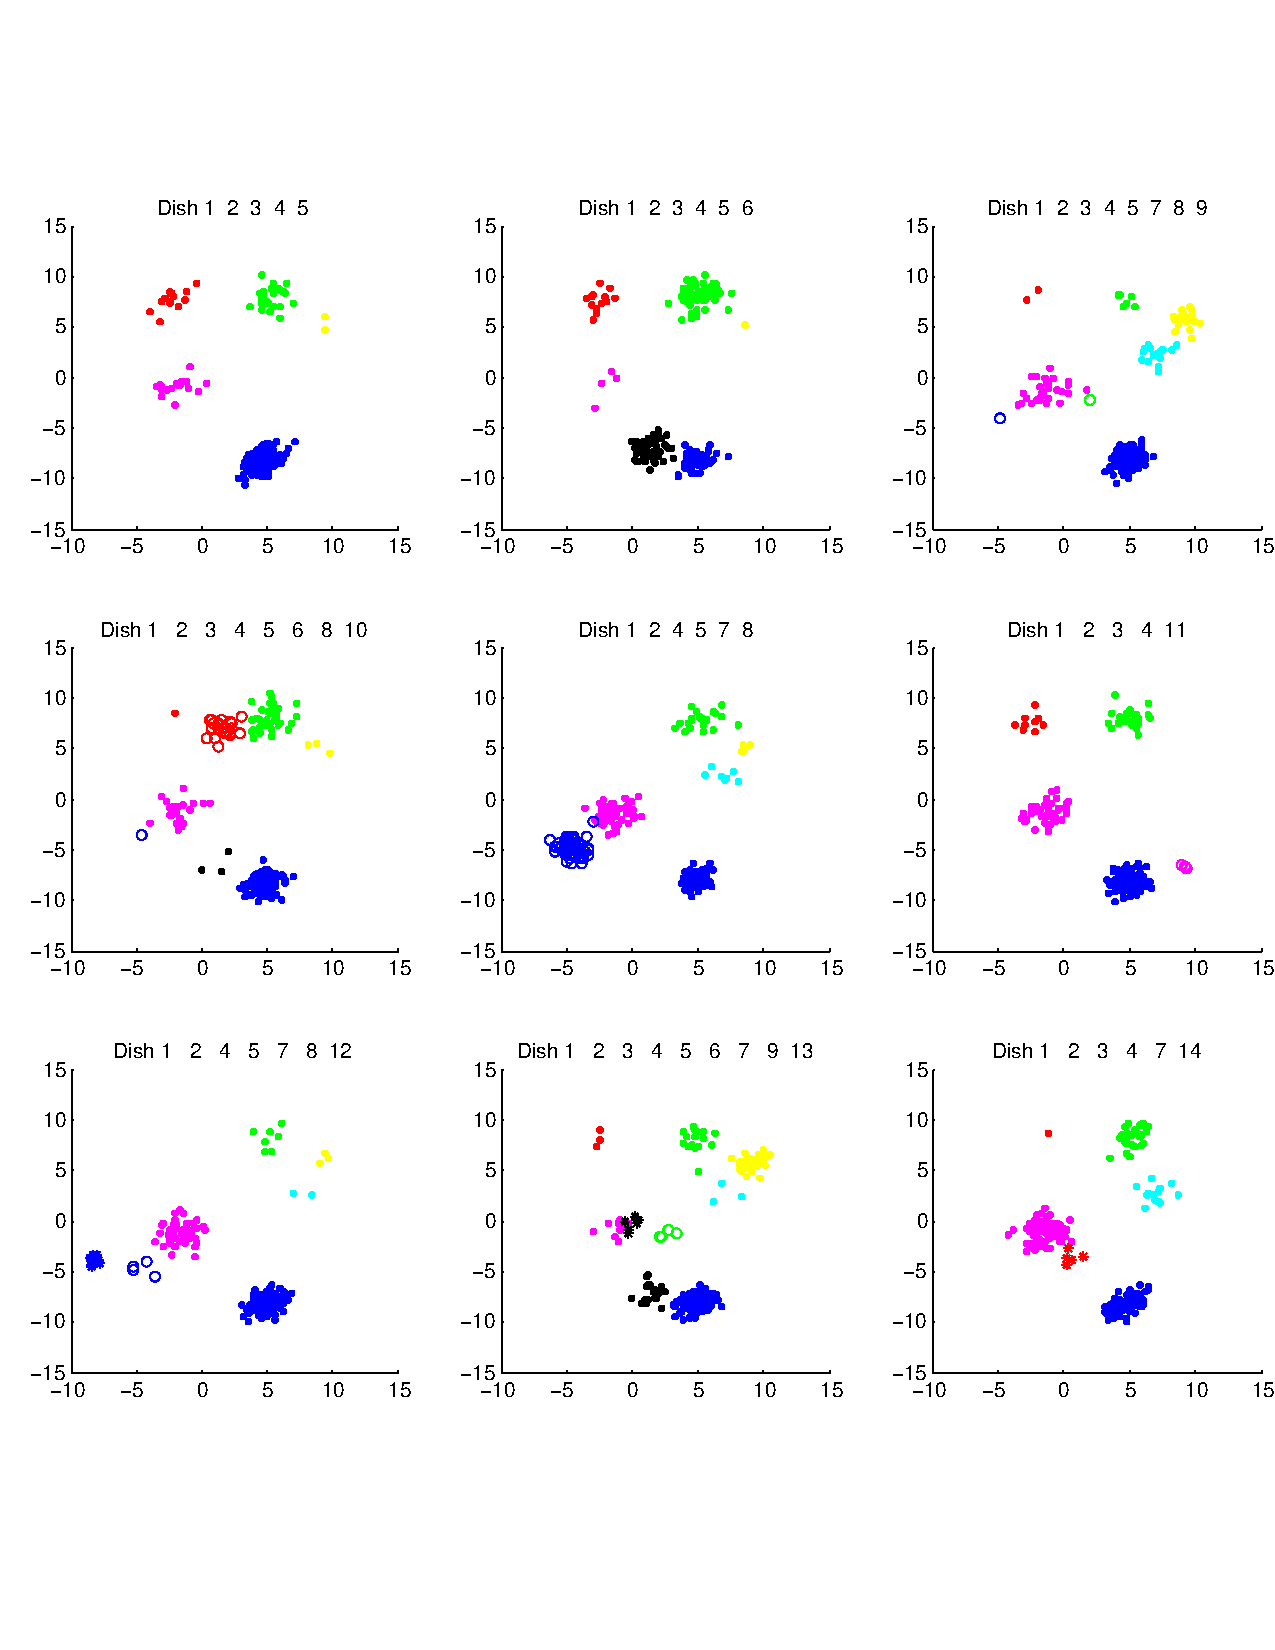
\includegraphics[width=3.5in,height=4.5in]{g_t.pdf} 
    \caption{9 Restaurants sharing same menu of dishes} 
    \label{fig:by:table} 
  \end{minipage}% 
  \begin{minipage}[b]{0.5\textwidth} 
    \centering 
    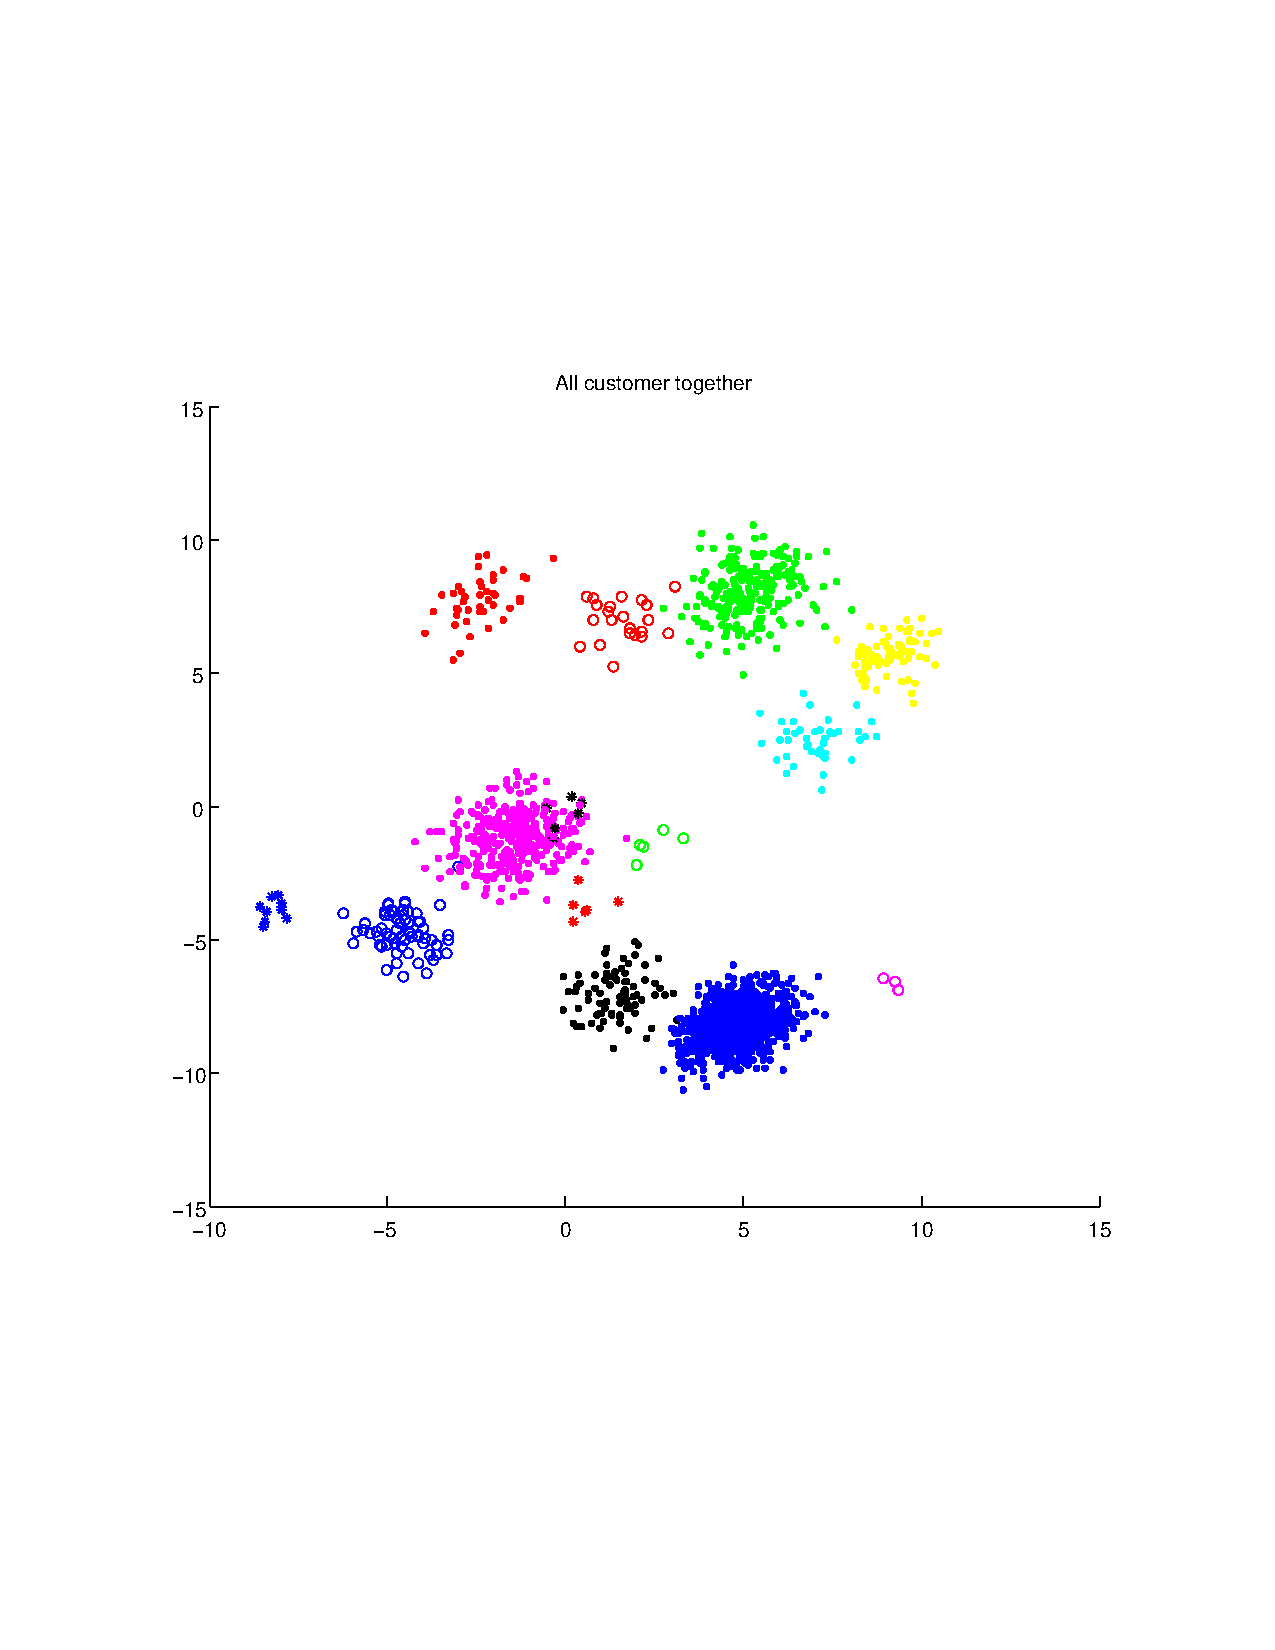
\includegraphics[width=3.5in,height=4.5in]{g_t2.pdf} 
    \caption{All customers together}
    \label{fig:by:table}  
   \end{minipage}% 
\end{figure}



\section{3. Search $\vec z$}
The Goal is to find the $\vec z$ which gives the highest marginal probability P=$p(x|z,\lambda)$.\\
\subsection{1) Local Search}
Heuristically, we first try out the local search.
\begin{enumerate}[(I)]
\item Outline:
\begin{enumerate}[(a)]
\item Initialization: Every customer has his own table and every table has its own dish
\item Iteration:\\
\\ While there are still some local changes to increase P:
\begin{enumerate}[(i)]
\item In Random order, assign every customer the table in his restaurant which increases P mostly conditioning on other cutomers unchanged
\item In Random order, assign every table the dish which increases P mostly conditioning on other tables unchanged
\end{enumerate}
end

\end{enumerate}
\item Result:\\
\begin{figure}[h] 
  \begin{minipage}[b]{0.5\textwidth} 
    \centering 
        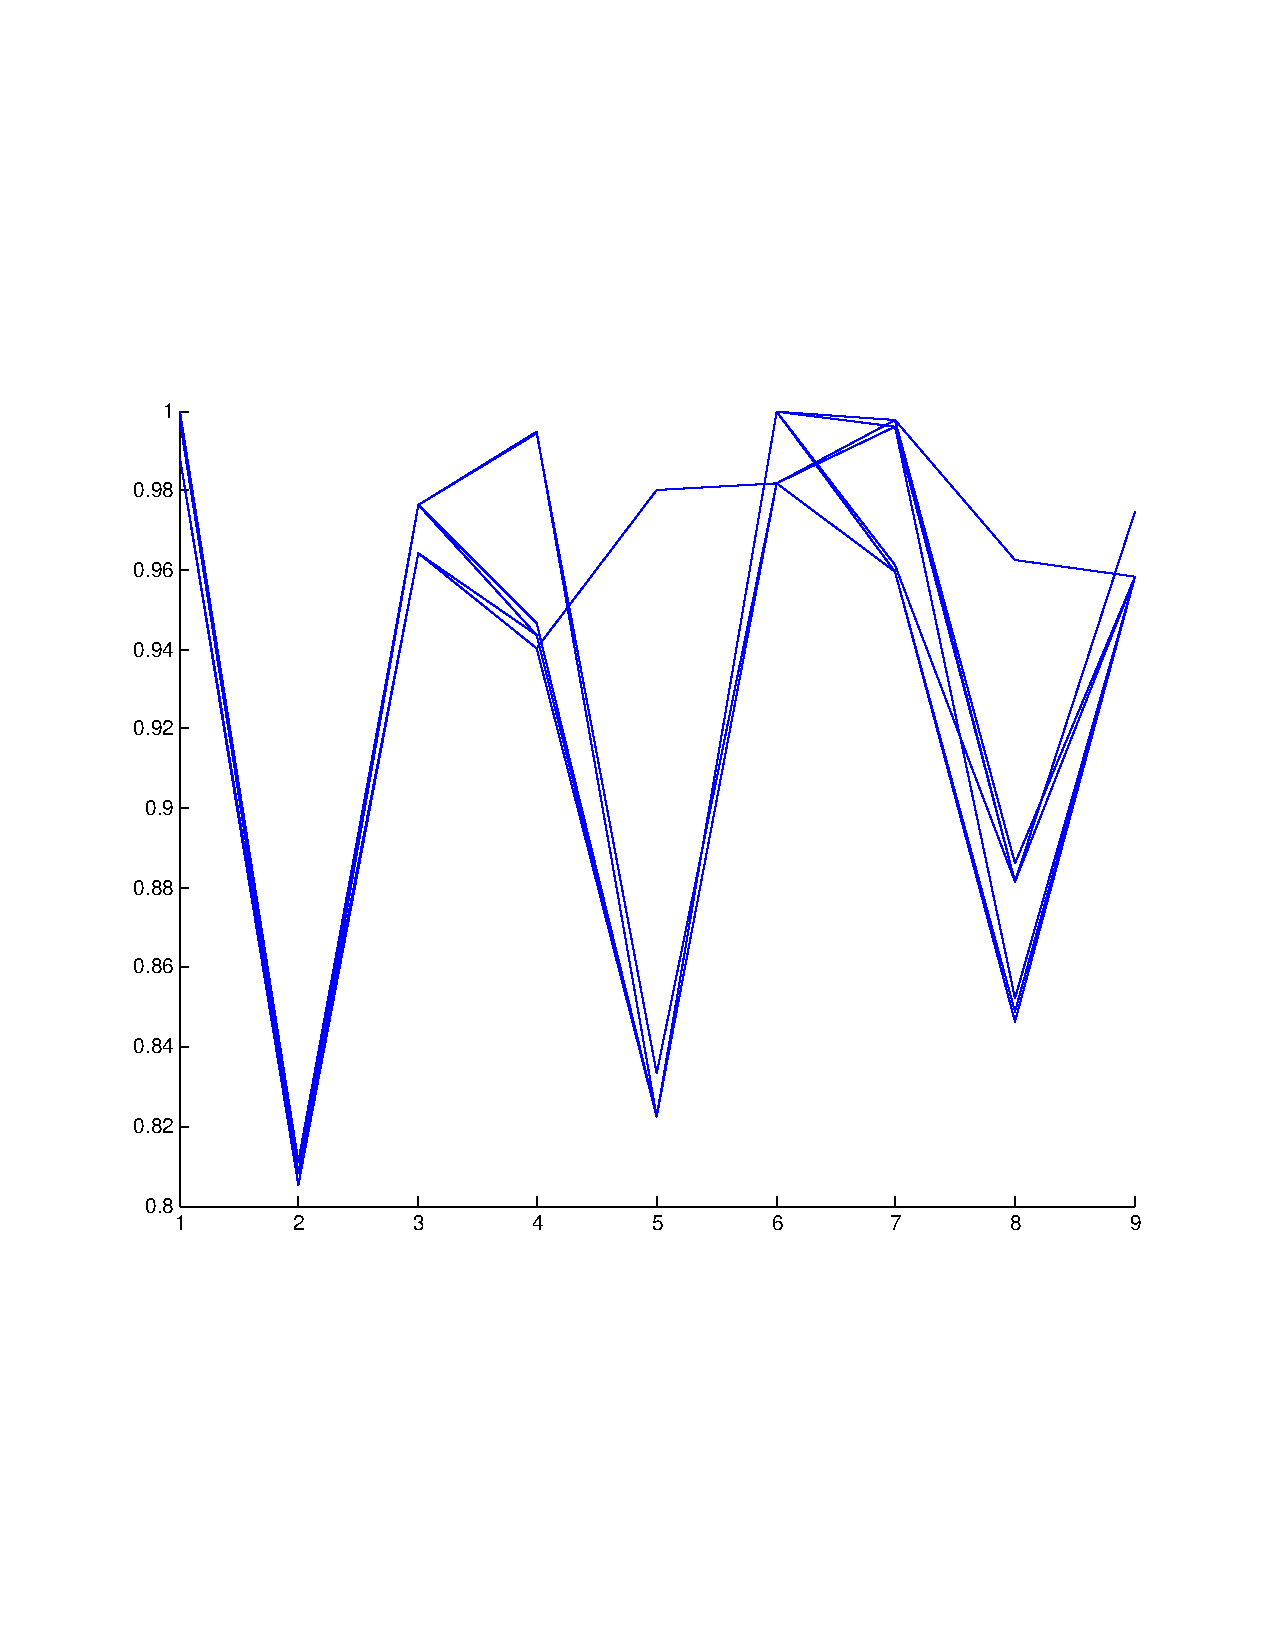
\includegraphics[width=3.5in,height=4.5in]{rand_lo.pdf} 
    \caption{random index for each restaurant of one random search order} 
    \label{fig:by:table} 
  \end{minipage}% 
  \begin{minipage}[b]{0.5\textwidth} 
    \centering 
    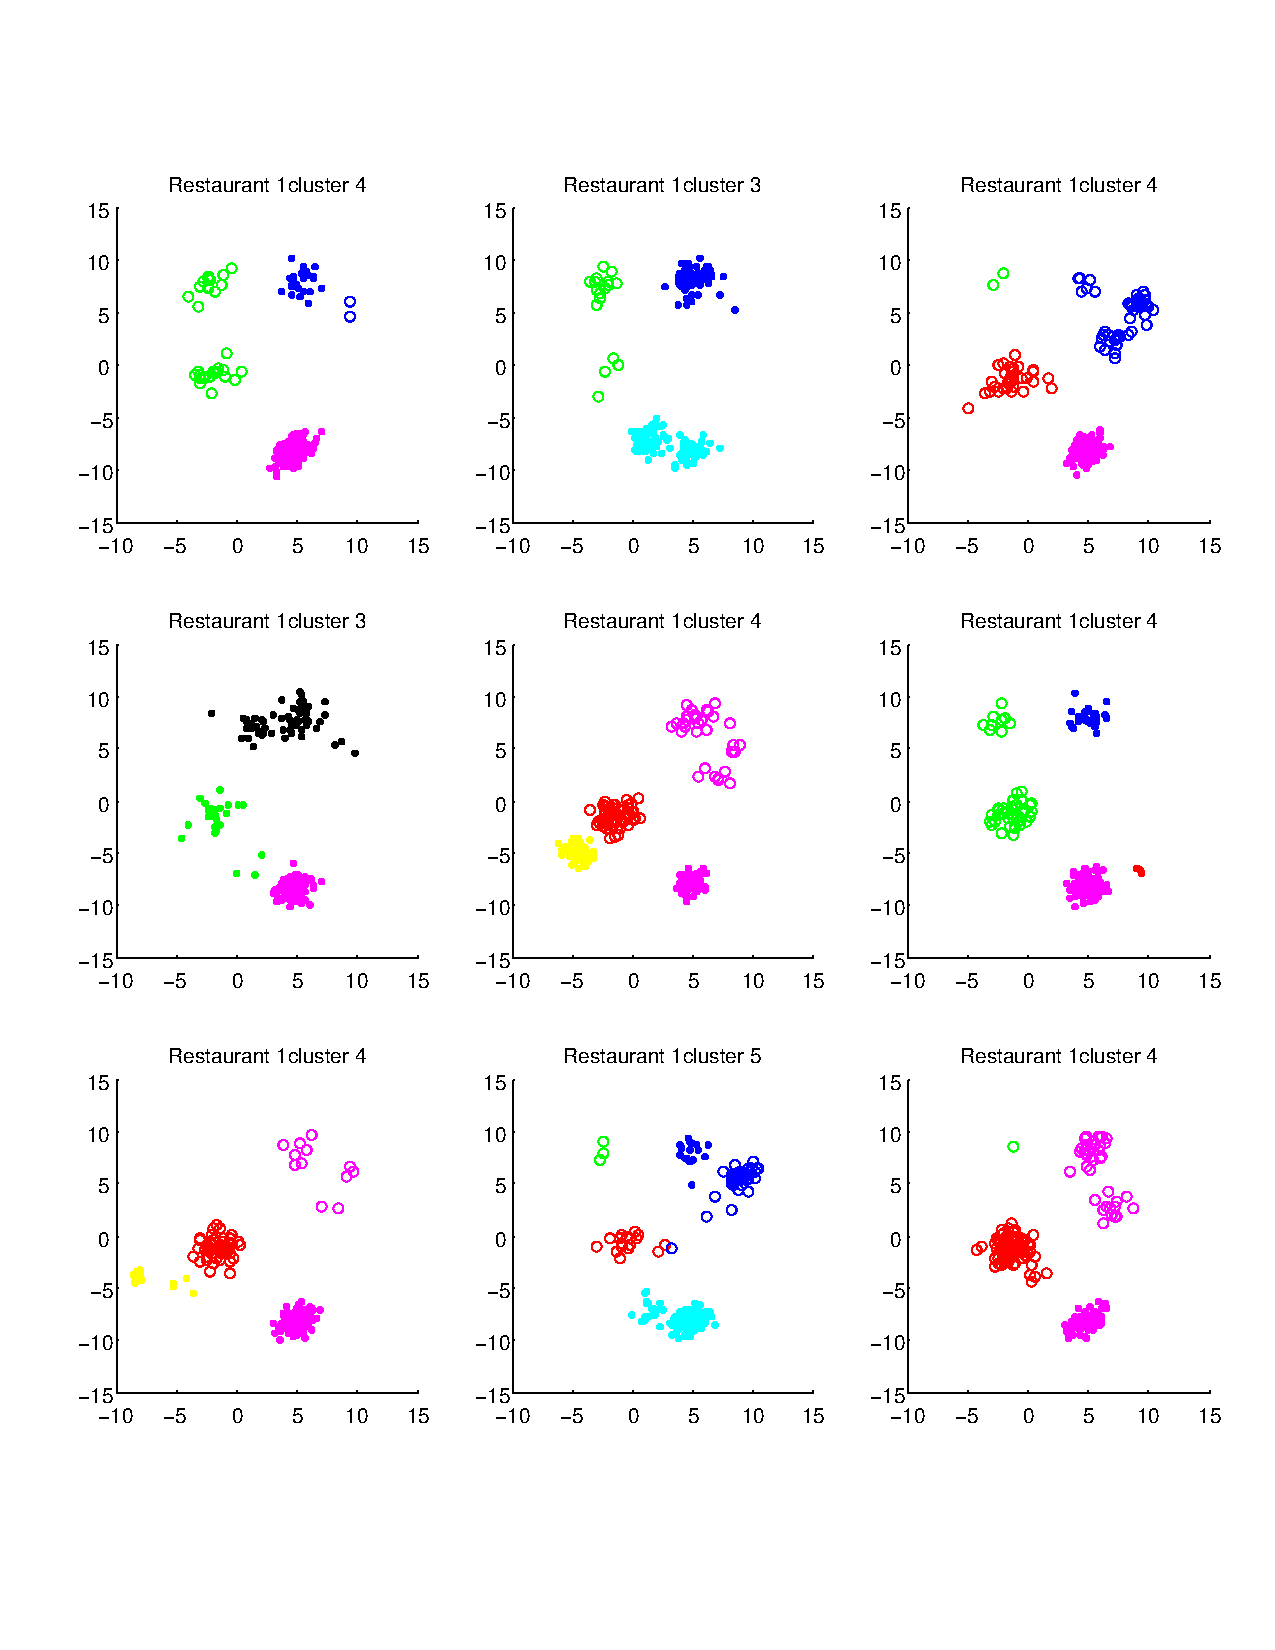
\includegraphics[width=3.5in,height=4.5in]{me_3.pdf} 
    \caption{cluster result of one random local search order}
    \label{fig:by:table}  
   \end{minipage}% 
\end{figure}
The clustering result for Restaurant 2,5,8 is not good enough, which have big clusters.
\end{enumerate}

\subsection{2) Local Search+Split$\&$Merge}
After local search gets stuck at a local maxima, we try out split and merge(bigger moves) to find better maxima.
\begin{enumerate}[(I)]
 \item Outline:
\begin{enumerate}[(a)]
\item Initialization: Start from the Fixed Point(local maxima) from Local Search
\item Iteration:\\
\\ While one of the last N moves of split or merge moves increases P:\\
Switch ceil(4*rand())
\begin{enumerate}[(i)]

\item case 1: In Random order, use k-means++ to split every dish into 2 dishes and accept it only if it increases P
\item case 2: In Random order, use k-means++ to split every table into 2 tables and accept it only if it increases P
\item case 3: In Random order, merge every dish to another one which increases P mostly conditioning on other dishes unchanged and reject it if all merge moves decrease P
\item case 4: In Random order, merge every table to another one in the same restaurant which increases P mostly conditioning on other tables unchanged and reject it if all merge moves decrease P
\end{enumerate}
end
\end{enumerate}



\item Result:
Cluster result of one random split$\&$merge order
\begin{center}[h] 
    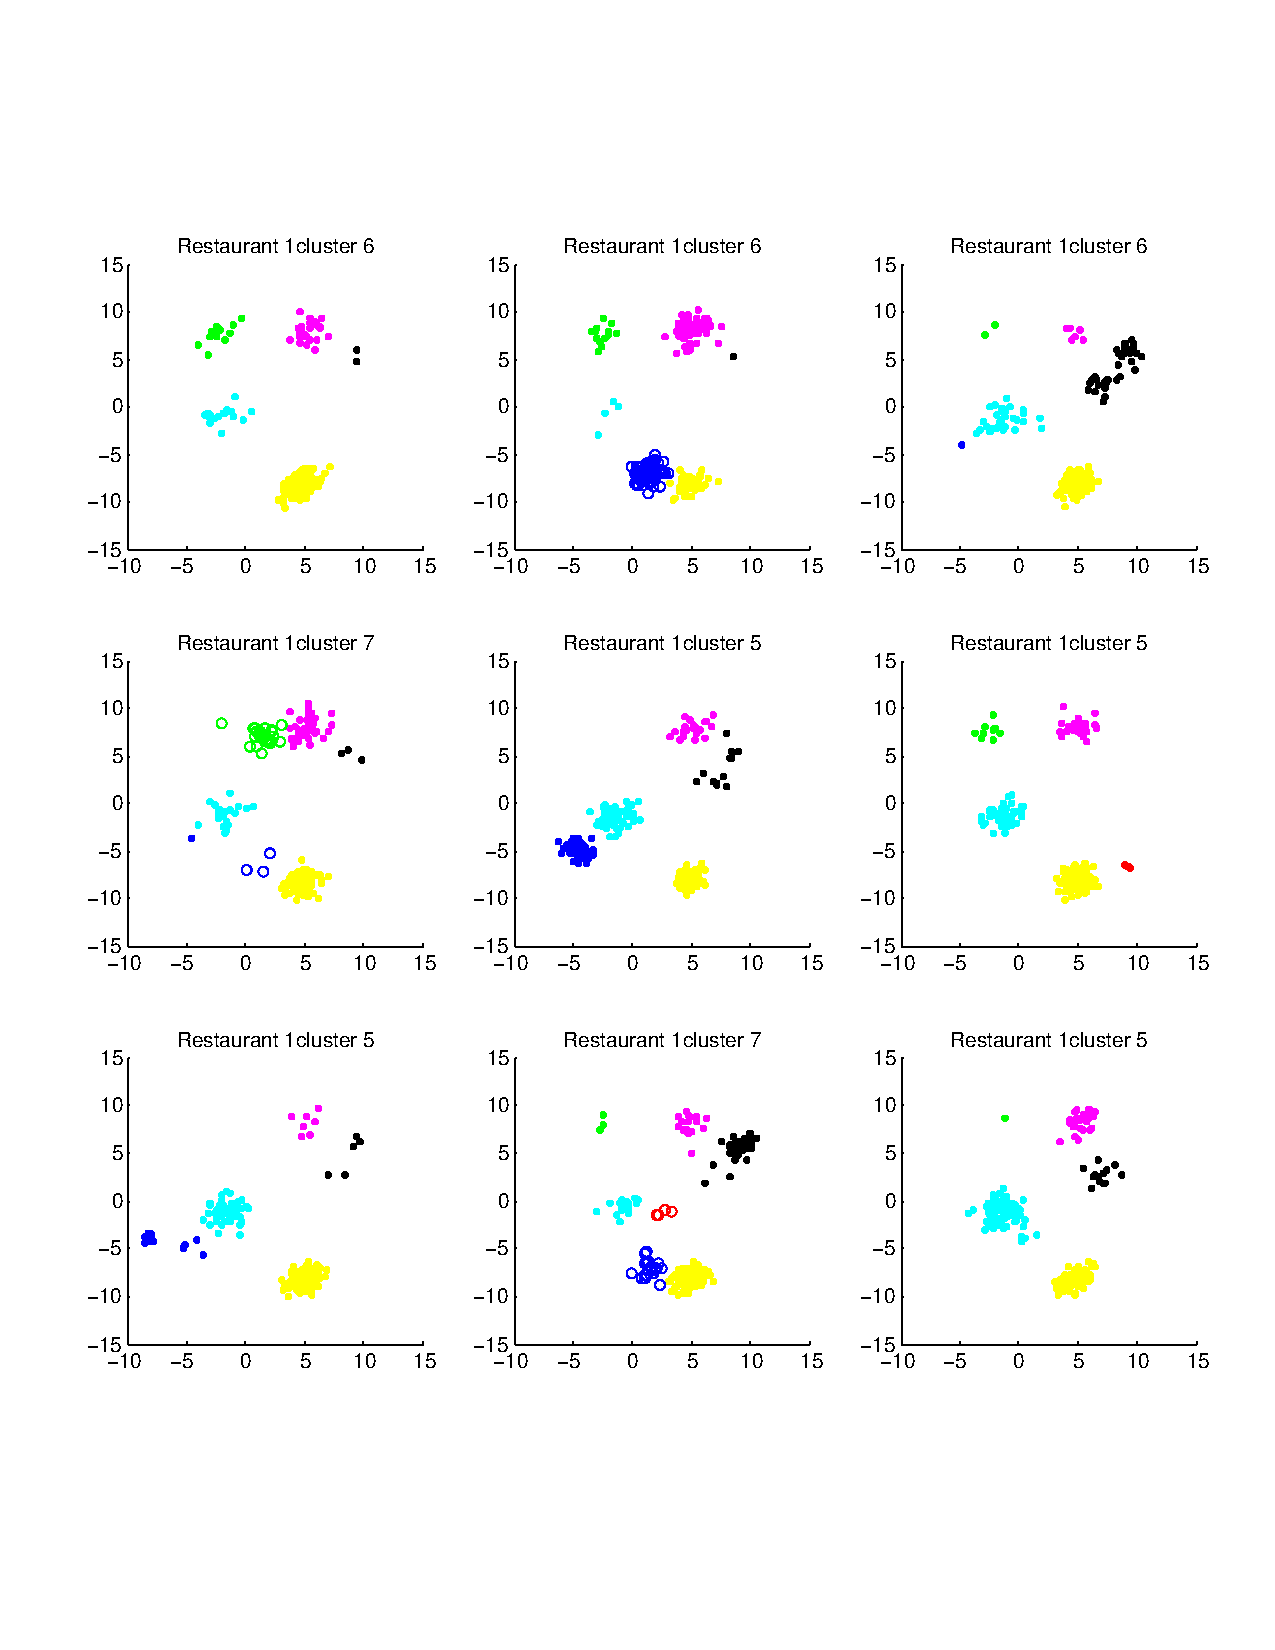
\includegraphics[width=5in,height=5in]{sm_1.pdf}
\end{center}

\begin{center} 
    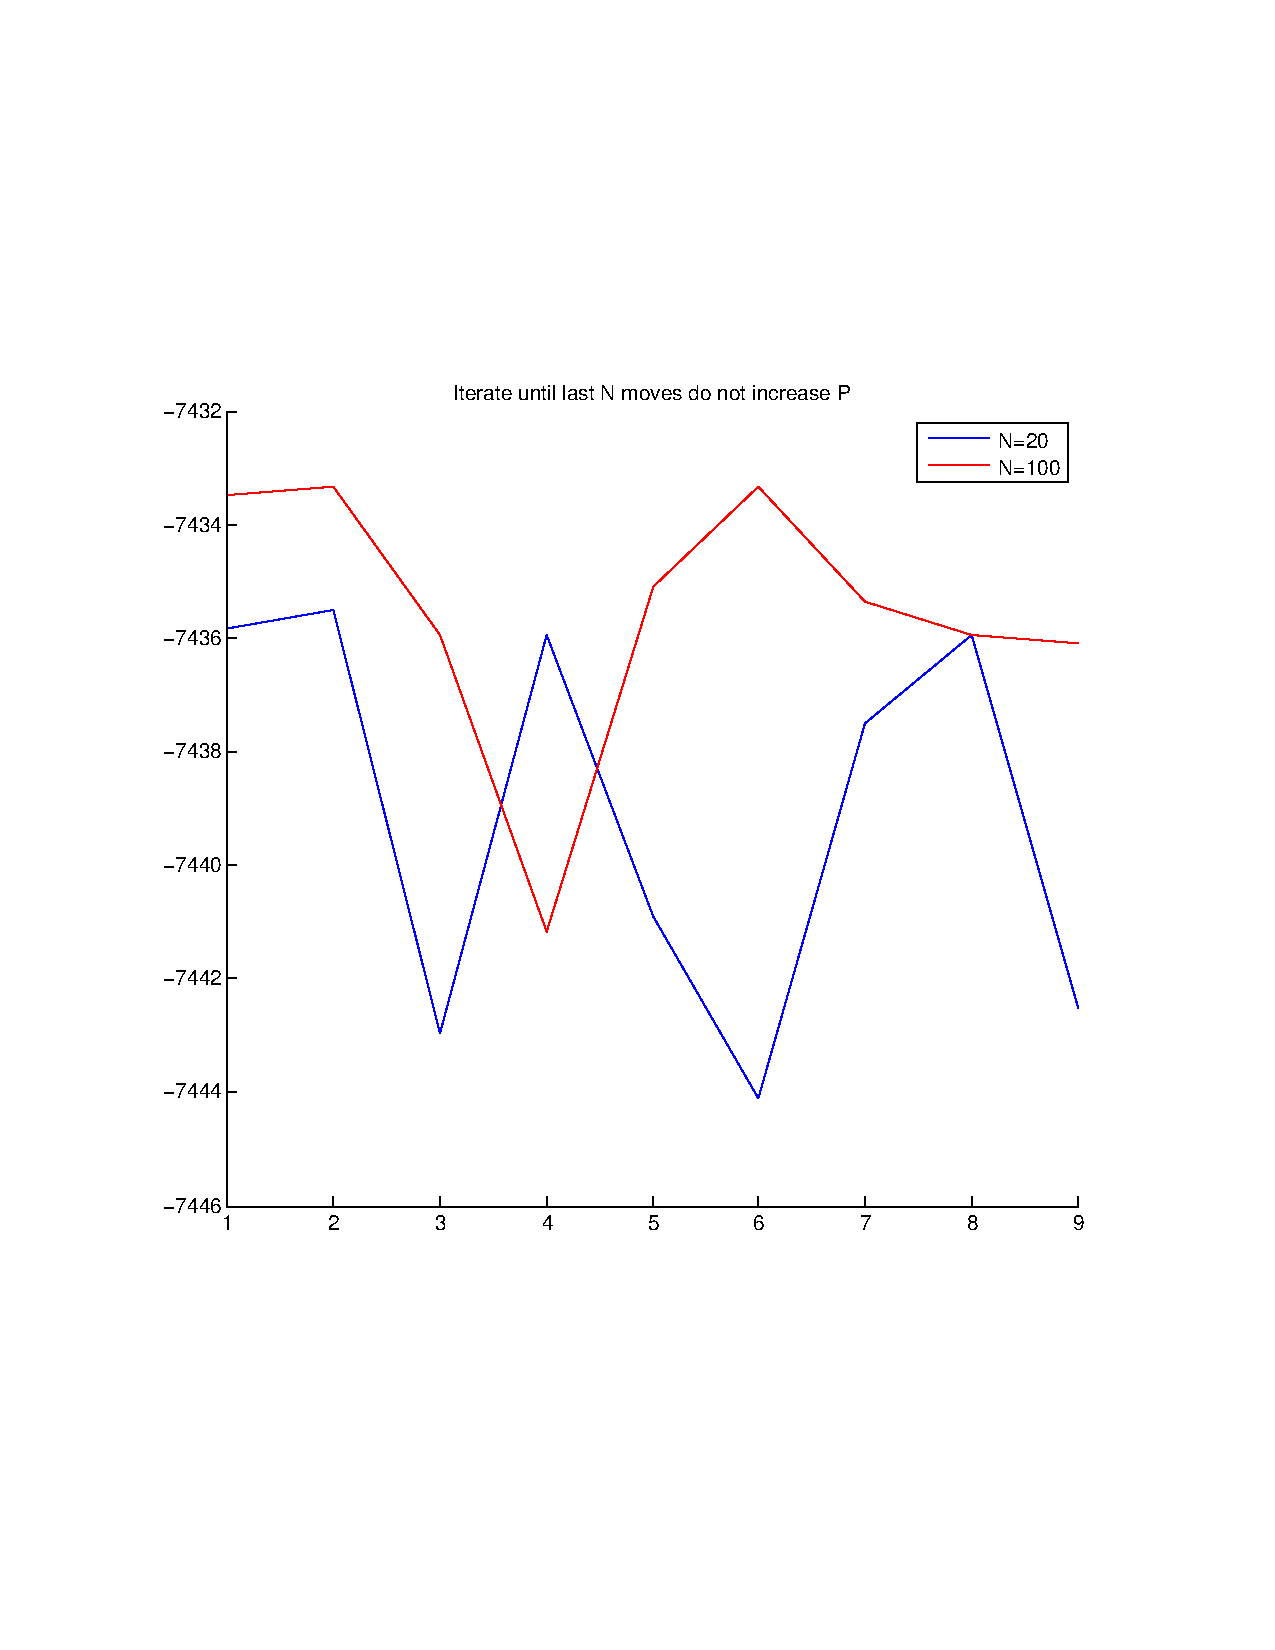
\includegraphics[width=3in,height=3in]{sm_com.pdf}
\end{center}

For Split$\&$Merge, we end the iteration until last N moves do not increase the log probability any more.We tried N=20 and N=100, which gives similar log probability.
\begin{figure}[h]
  \begin{minipage}[b]{0.5\textwidth} 
    \centering 
        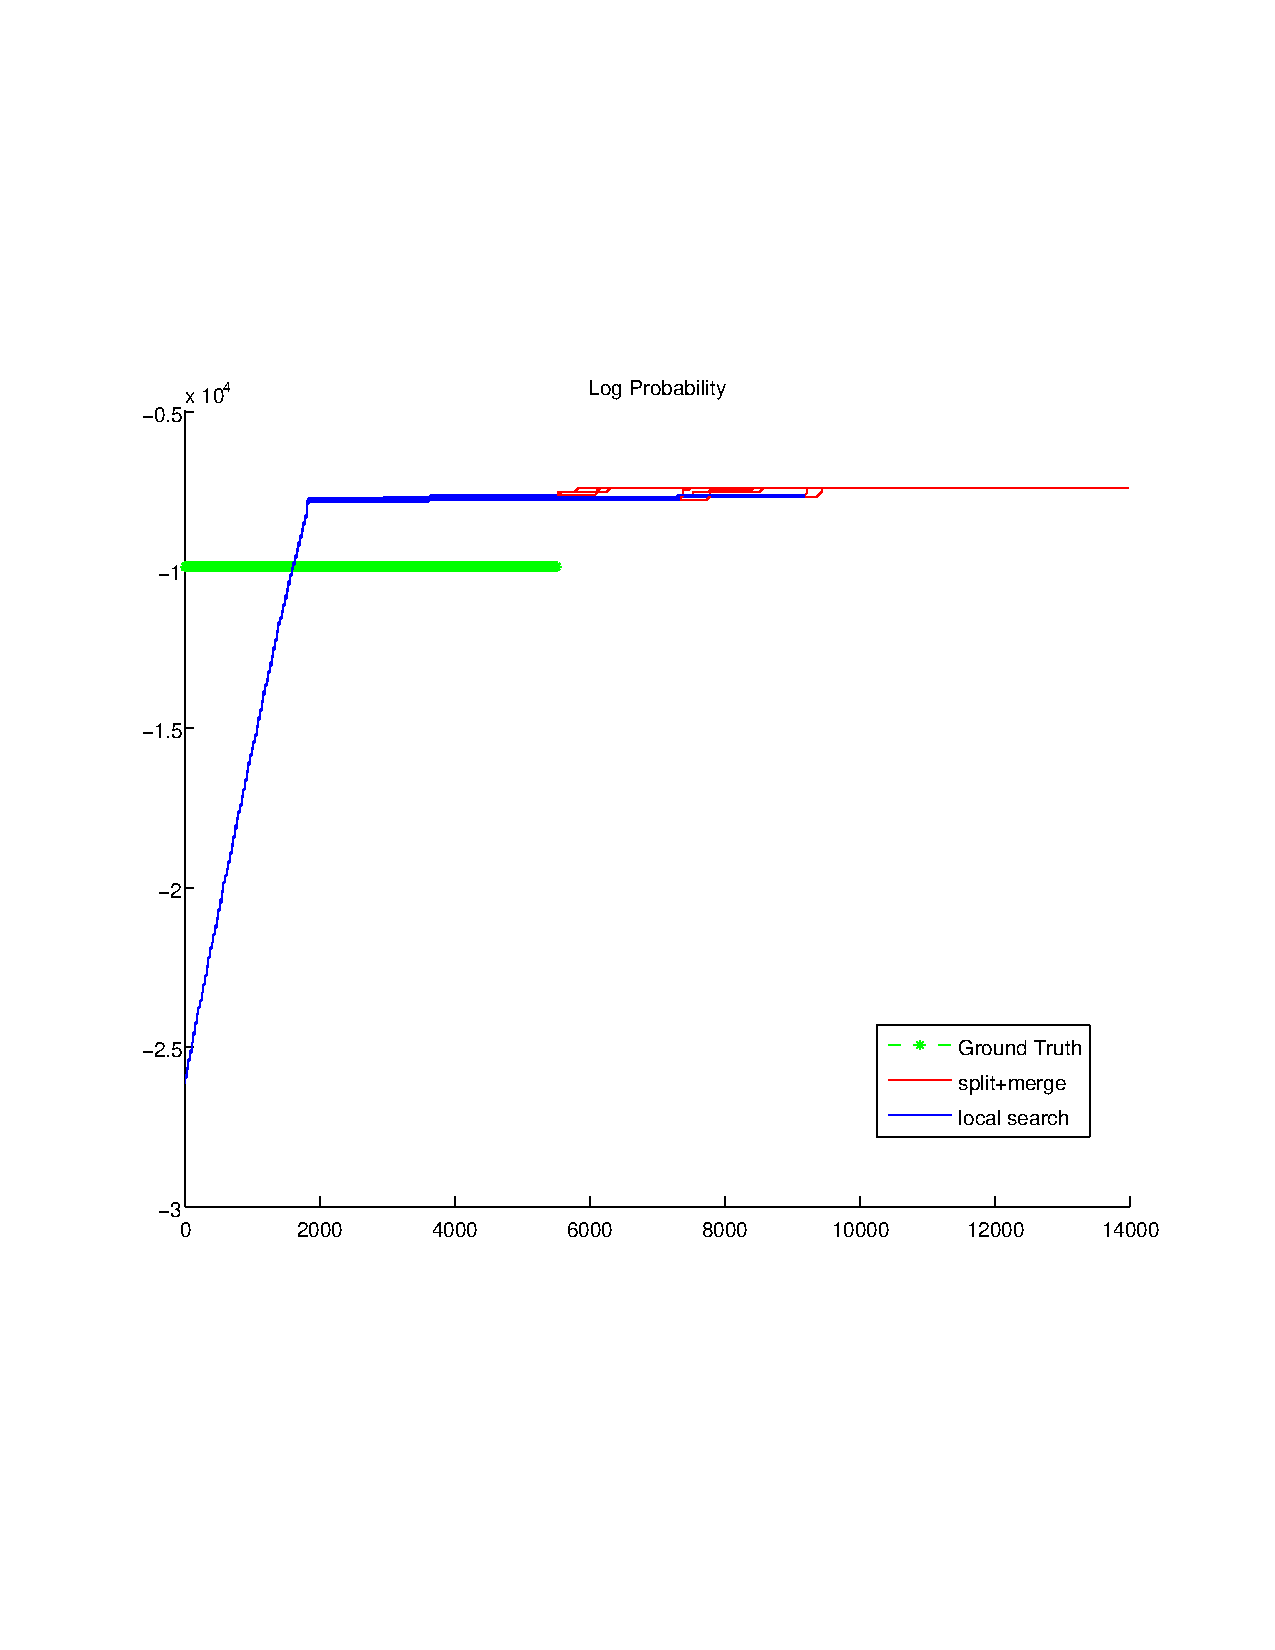
\includegraphics[width=3.5in,height=4.5in]{log_prob.pdf} 
    \caption{Log probability v.s. Steps} 
    \label{fig:by:table} 
  \end{minipage}% 
  \begin{minipage}[b]{0.5\textwidth} 
    \centering 
    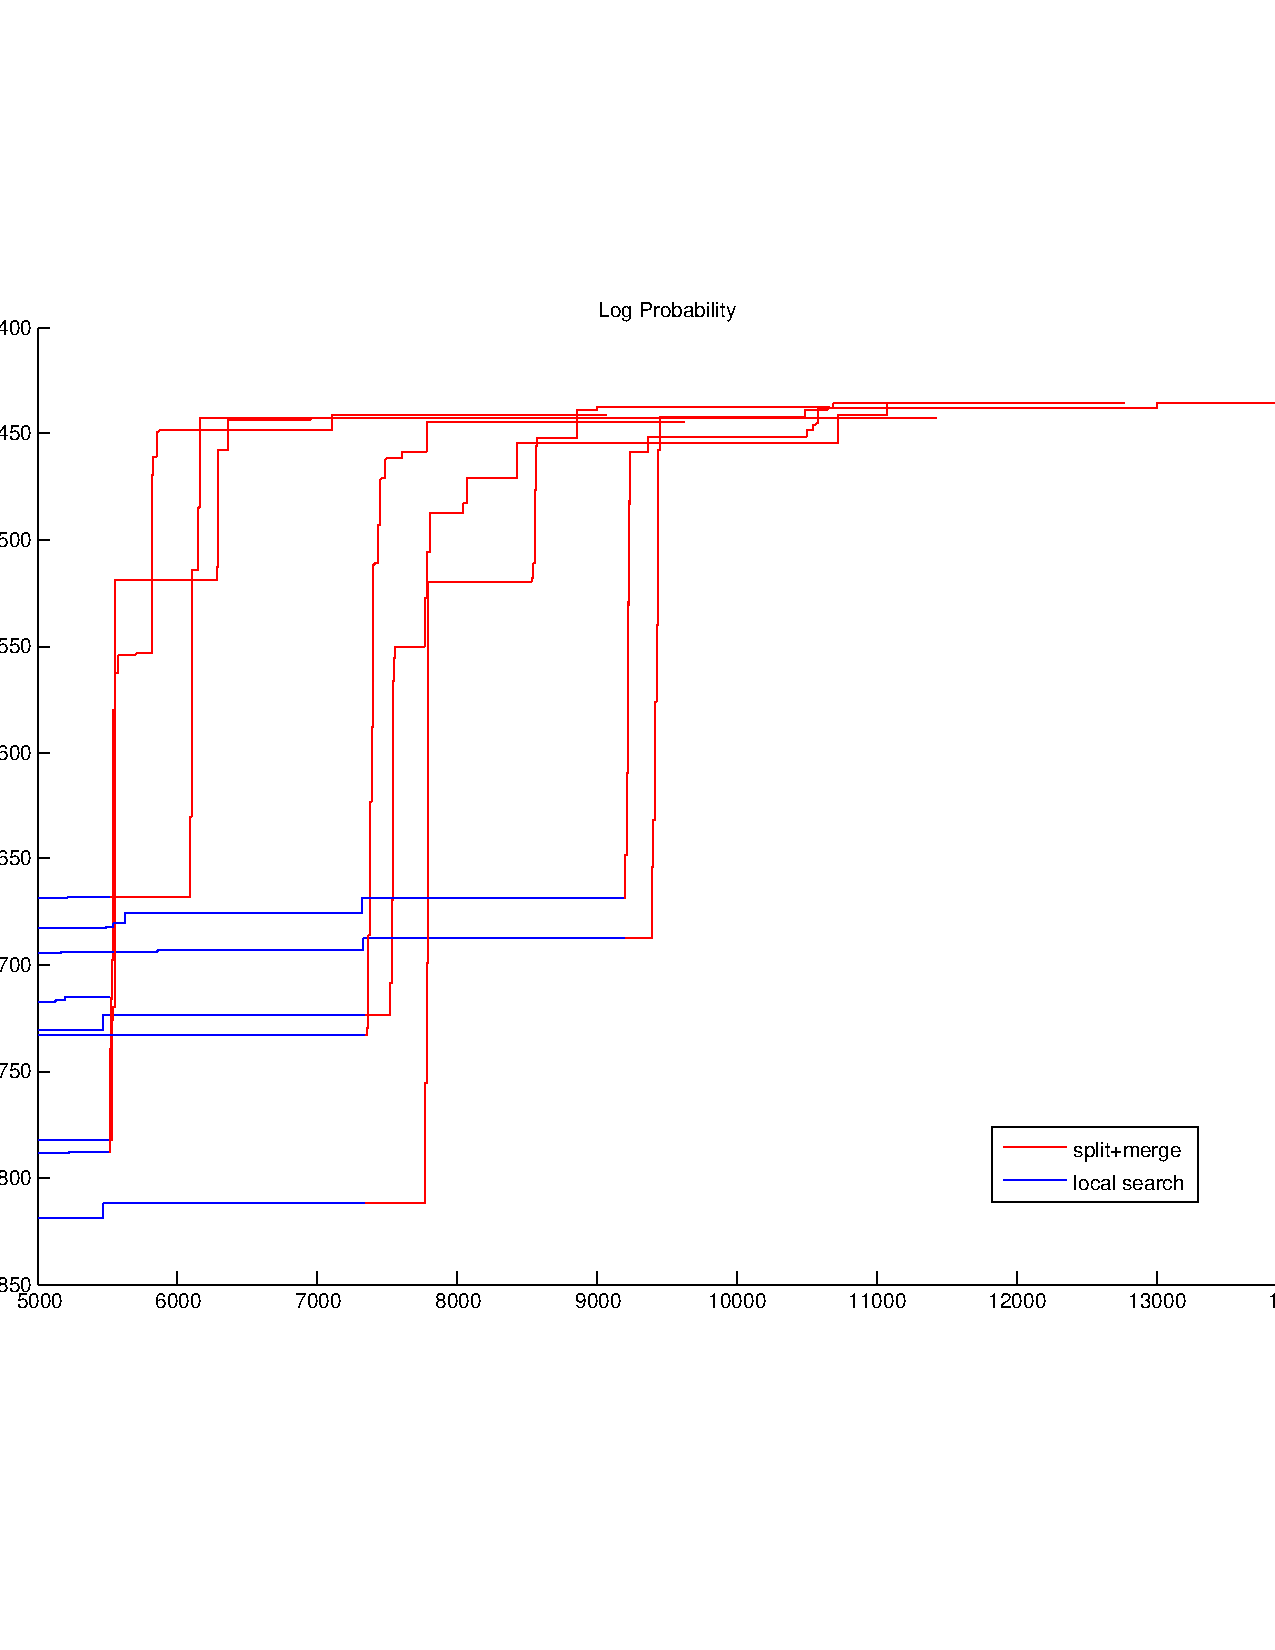
\includegraphics[width=3.5in,height=4.5in]{log_prob_2.pdf} 
    \caption{Closer LOOK of the convergence of log probability by split $\&$ merge}
    \label{fig:by:table}  
   \end{minipage}% 
\end{figure}
\begin{figure}[h] 
  \begin{minipage}[b]{0.5\textwidth} 
    \centering 
        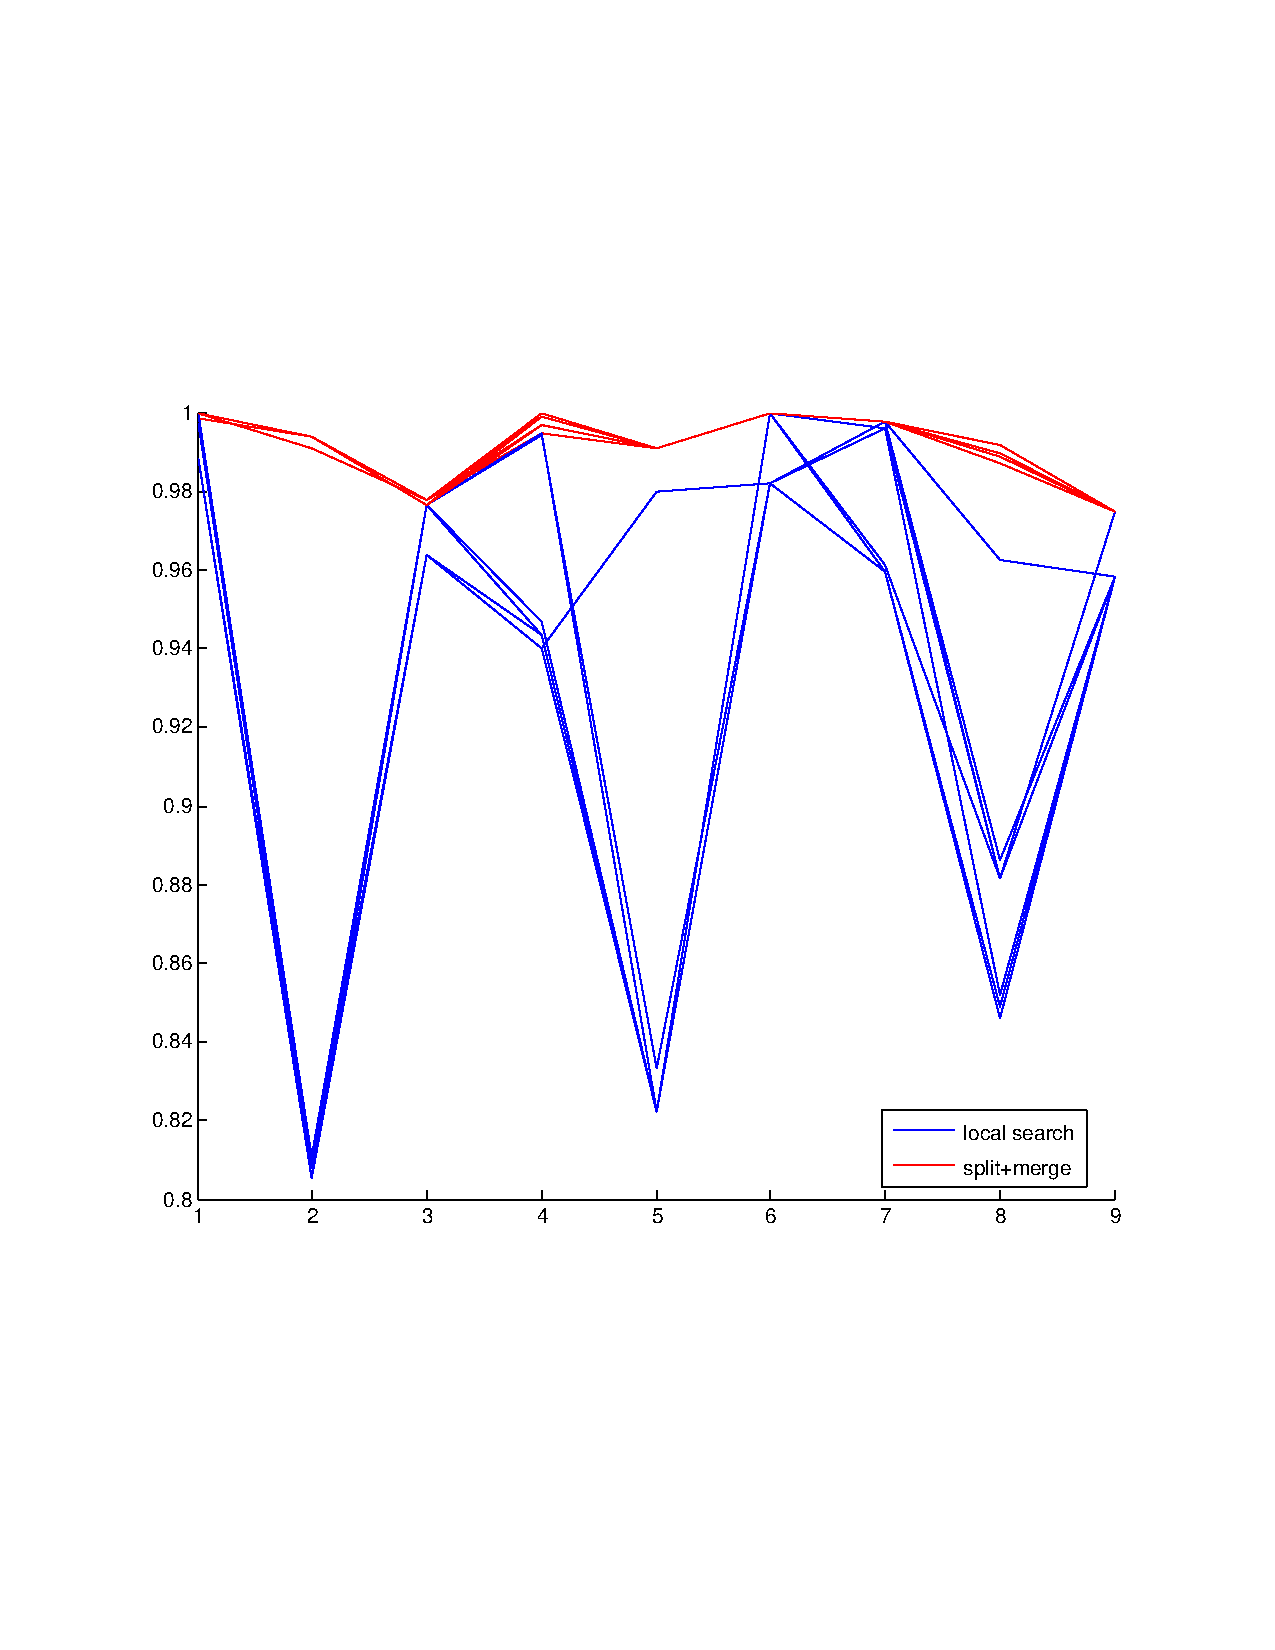
\includegraphics[width=3in,height=3in]{randin.pdf} 
    \caption{Rand Index Improvement Comparison} 
    \label{fig:by:table} 
  \end{minipage}% 
  \begin{minipage}[b]{0.5\textwidth} 
    \centering 
    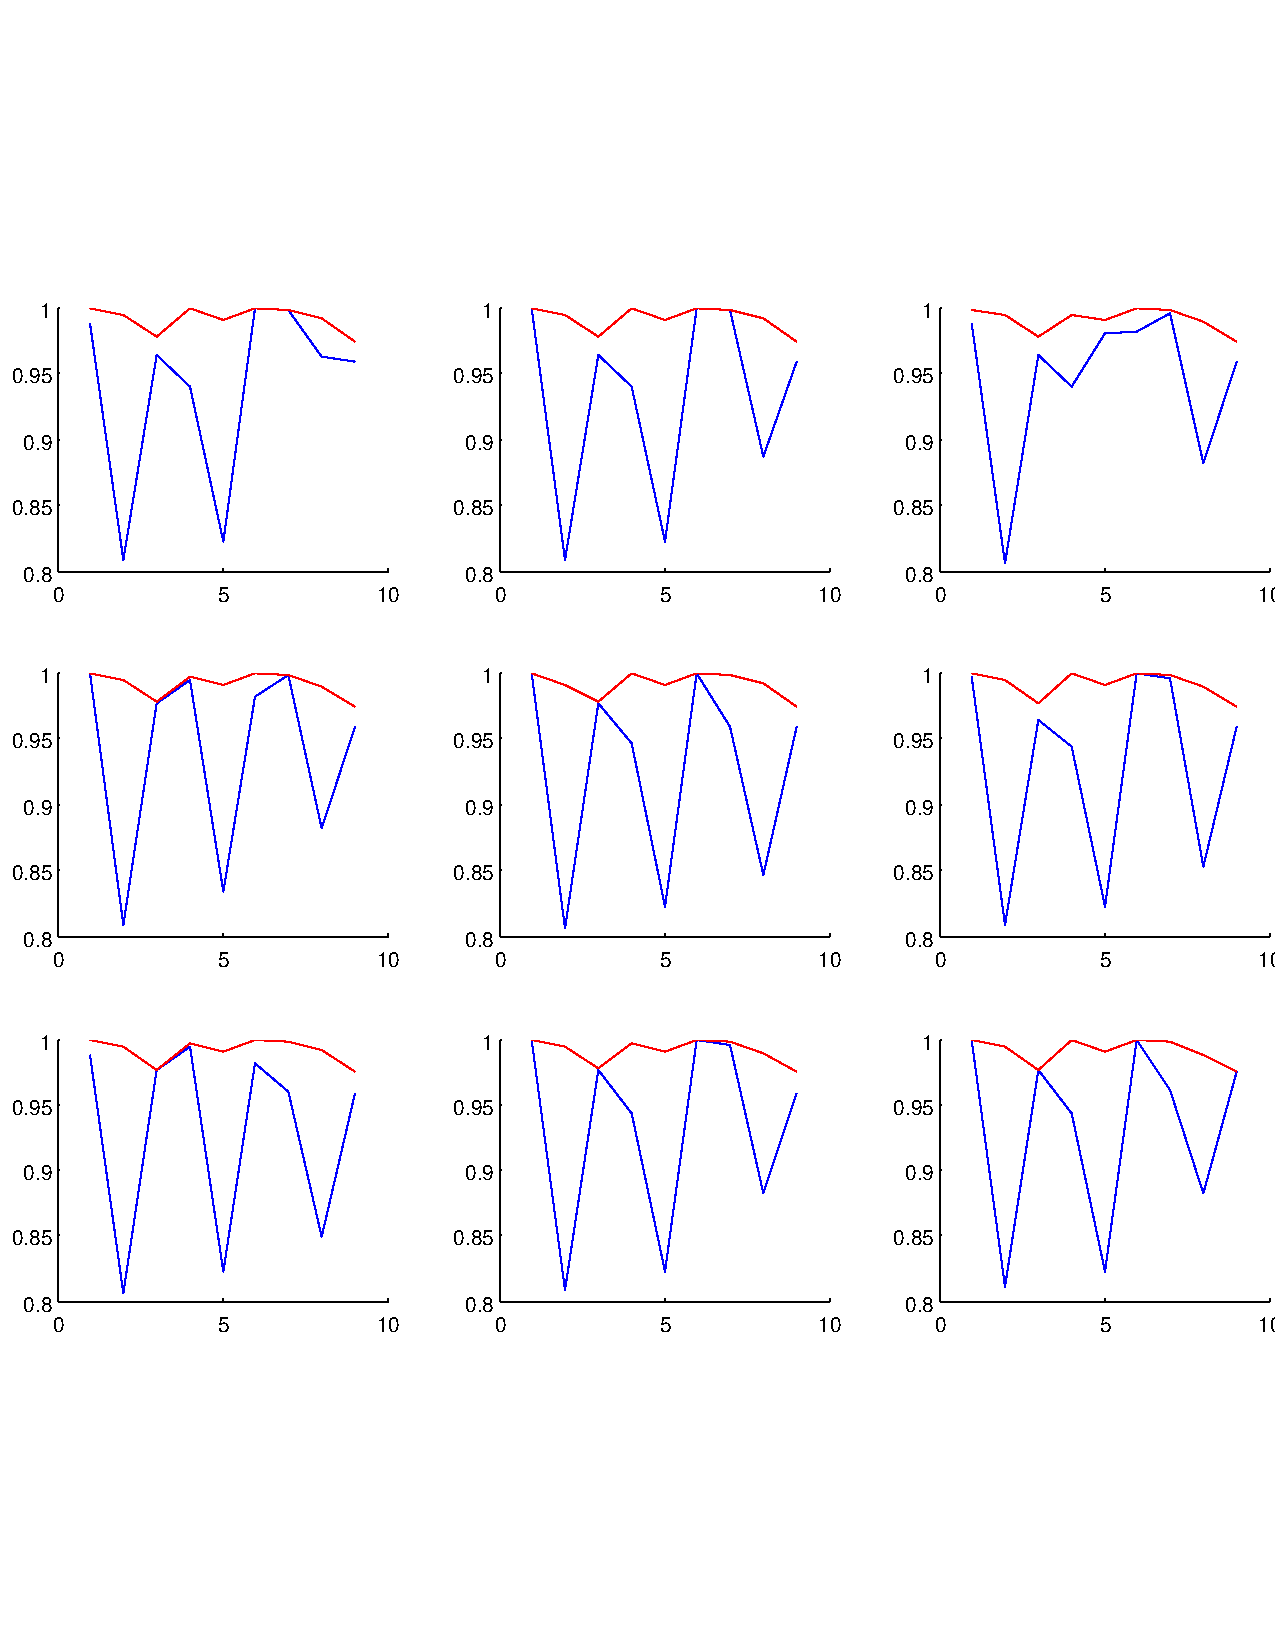
\includegraphics[width=3in,height=3in]{randin_2.pdf} 
    \caption{Rand Index Improvement in each restaurant}
    \label{fig:by:table}  
   \end{minipage}% 
\end{figure}


\end{enumerate}

\end{spacing}
\end{document}

%%%%%%%%%%%%%%%%%%%%%%%%%%%%%%%%%%%%%%%%%%%%%%%%%%%%%%%%%%%%%
